% This is an example for a `Introduction'.
% To generate the final document, run latex, build and quick build commands
% on the skeleton-thesis file not this one.

\chapter{Introduction}\label{chapters:Introduction}
\vspace{-7mm}

While seemingly small objects, nuclei and their interactions can play an enormous role across a wide swath of energy and spatial scales.
From understanding the abundance of elements produced in astrophysical events to providing a general description of quantum many-body equilibration, the deceptively simple study of two colliding nuclei can be illuminating.
Even the more traditionally aligned investigations that are associated with nuclear reactions (such as superheavy element and neutron-rich nuclei formation) acts as a foundation for other areas of physics to piece together an understanding of the physical world.

Leaving aside the fact that nuclei are made of protons and neutrons, the dynamics of interacting quantum systems alone is of extreme interest to researchers from varied fields.
This is due to the striking fact that most quantum many-body systems (no matter the specific systems and particles that compose their structure) exhibit the same general features as atomic nuclei.
That is to say that studying the fusion, transfer, equilibration, vibrations, etc. of nuclear systems can provide vital insight into analogous studies in interactions between cold atoms or molecules -- systems which are several orders of magnitude larger than the few femtometers (fm) of interest to nuclear physicists.

\section*{The Nuclear Many-Body Problem (in a nutshell)}

\begin{figure}[t]
	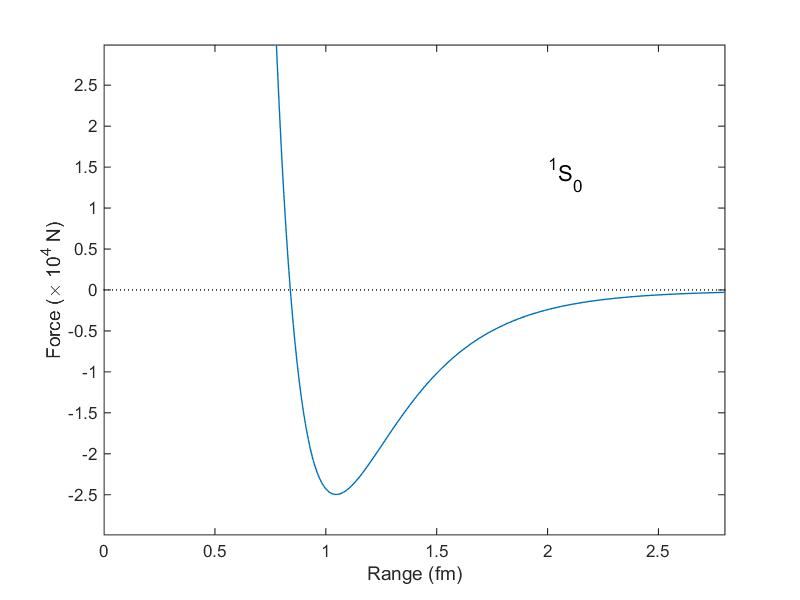
\includegraphics[width=\textwidth]{../Figures/intro_figs/ReidForce2.jpg}
	\caption{An example nucleon-nucleon potential from the Reid model~\citep{reid1968} of the nuclear force. Note the characteristic exponential decay in the attractive tail, as well as the strong repulsion that tends toward infinity at $R\approx0.7$. Figure from~\citep{bdushaw}.}
	\label{fig:reid}
\end{figure}

The specific subbranch of nuclear physics this thesis focuses on is the realm of low-energy nuclear physics.
At this level, relativistic effects are typically neglected and the nuclei are modeled as collections of protons and neutrons interacting with each other to form a bound system.
The force felt by the nucleons themselves is an artifact of the strong interaction, mediated primarily by the exchange of virtual pions with an effective range of about~$1$~fm.
Through further contributions by vector mesons (principally rho and omega), a complicated model of interacting nucleons can be built that depends on not only a nucleon's charge and distance, but also on its spin and angular momentum as well.
An example channel of the Reid potential~\citep{reid1968} is shown in Fig.~\ref{fig:reid}.
Extensive effort has been placed in modeling nuclei using such an interaction (see ~\citep{wiringa1995} for another popular choice of an N-N potential), though this \textit{ab initio} approach is not numerically feasible for large nuclei or for simulating dynamical interactions between nuclei.
It is for this reason that alternate approaches to modeling finite nuclei have been pursued throughout the field's history.

One such approach is that of the mean-field method which, simply stated, assumes that each nucleon moves freely through an average field made up of contributions from all the other nucleons.
This independent particle approximation is extremely powerful because it reduces a series of N-body self interactions to a simple sum over each individual particle.
%in the mean-field.
%A schematic image is shown in Fig.~\ref{fig:meanfield}.
While many takes on the mean-field idea have been pursued over time, the foundation of the current work was formulated in 1928 when Hartree developed the self-consistent field method~\citep{hartree1928}.
This was further extended for antisymmetric systems by Fock to form the more complete Hartree-Fock method that has been used since~\citep{fock1930}.
The term "self-consistent" used above refers to the fact that the effective Hamiltonian of the system depends on the single particle wave functions themselves, thus requiring the problem to be solved iteratively.
One common approach is to choose an initial guess of Gaussian wave packets for the first step and then a minimization procedure is followed to obtain the ground state solution for the nucleus.
Despite having a general purpose algorithm for self-consistently solving the static many-body quantum problem, the method wasn't widely adopted until computational abilities were readily available due to the large matrices involved in larger systems paired with the iterative nature of the problem.


While the Hartree-Fock method provides a general purpose, robust numerical algorithm, it is only useful for studying static properties of nuclei.
To obtain a time-dependent theory based on the mean-field approximation, one may proceed in several ways\footnote{For a more complete description of the various approaches to deriving TDHF (including a path integral formulation, many-body perturbation theory, the Balian-V\'en\'eroni variational principle, etc) see~\citep{simenel2018}.} though we will focus on the derivation by minimization of the Dirac action.
As it's vital to all chapters of this thesis and reveals much about the approximations and limitations of the theory, I will cover the derivation in detail.
First, consider the Dirac action from $t_0$ to $t_1$,
\begin{equation}
S\equiv S_{t_0,t_1}[\Psi] = \int_{t_0}^{t_1}dt \langle \Psi(t) | \left(i\hbar\frac{d}{dt}-\hat{H}\right)|\Psi(t)\rangle.
\end{equation}
For a generic many-body wave function, $|\Psi(t)\rangle$, the stationary solution of the action will simply be the Schr\"odinger equation, thus we impose that the many-body wave function is a Slater determinant of independent particle states $|\phi_i(t)\rangle$ to obtain
\begin{equation}
S_{t_0,t_1}[\Psi] = \int_{t_0}^{t_1}dt \left(\sum_{i=1}^{N} \langle\phi_i(t)|i\hbar\frac{d}{dt}|\phi_i(t)\rangle-\langle\phi_i(t)|\hat{H}|\phi_i(t)\rangle\right).
\end{equation}
This can be simplified further by defining the quantity $\sum_{i=1}^{N}\langle\phi_i(t)|\hat{H}|\phi_i(t)\rangle$ as an energy density functional (EDF), $E[\rho(t)]$.
Now, by varying with respect to single particle states we may impose the stationarity of the action
\begin{equation}
\frac{\delta S}{\delta\langle\phi_i(t)|}=i\hbar\frac{d}{dt}|\phi_i(t)\rangle - \int_{t_0}^{t_1}dt' \frac{\delta E[\rho(t)]}{\delta\langle\phi_i(t)|} = 0,
\end{equation}
with the final step being to utilize the chain rule in the EDF integral and define a final quantity, the single particle Hamiltonian, $h[\rho(t)]=\frac{\delta E[\rho(t)]}{\delta\rho(t)}$.
Collecting all of this, we are left with our final TDHF equation
\begin{equation}
i\hbar\frac{d}{dt}|\phi_i(t)\rangle = h[\rho(t)]|\phi_i(t)\rangle.
\label{eq:tdhf}
\end{equation}
By examining the form of the TDHF equations, we see that we have a description of the time evolution for each state, $i$, in the system.
Furthermore, the single particle Hamiltonian has a dependence on $\rho(t)$ and thus on the wave functions themselves.
This is in line with the self consistency feature of static Hartree-Fock mentioned above, and thus in the time propagation procedure densities from a half time step are typically used for stability.

\begin{figure}[t]
	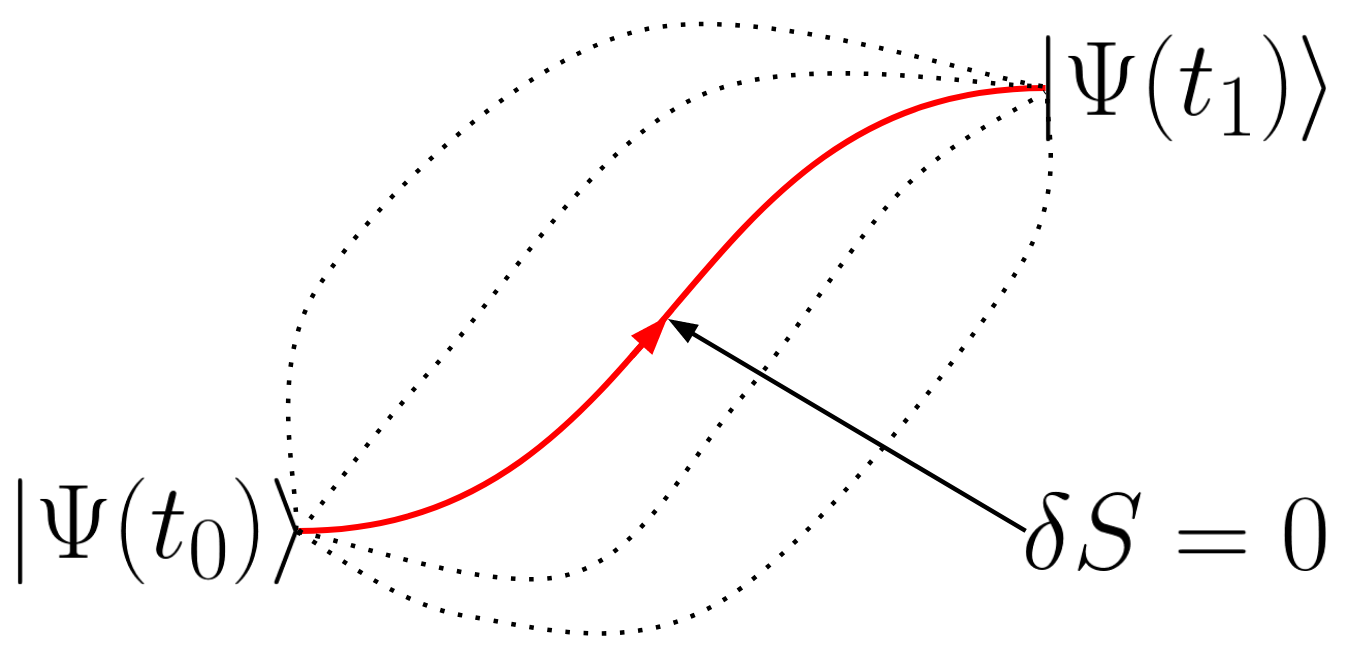
\includegraphics[width=\textwidth]{../Figures/intro_figs/paths.png}
	\caption{A schematic depiction of the stationary path chosen for the TDHF evolution.}
	\label{fig:paths}
\end{figure}

An extremely important feature of the TDHF method comes about by restricting ourselves to the stationary path from $t_0$ to $t_1$, namely that we recover only a single path in time.
This is at odds with a fully quantum picture of a many-body system evolving in time where multiple paths have some probability of occurring.
Figure~\ref{fig:paths} shows a schematic explanation of this choice.
It is for this reason that TDHF is described as a semi-classical theory and only recovers the most probable event in a time evolution.
Beyond this, the derivation required us to consider fully independent particles, just as assumed in the Hartree-Fock method, meaning that many-body correlations will not be considered.
As will be seen later in this thesis, these (and other) limitations require extensions to the base theory to uncover features in nuclear reactions that are absent with the present formulation.
Despite the theoretical shortcomings of the approach, pure TDHF calculations have been extremely successful in reproducing experimental data over its history.

One final point of interest to note from the derivation above is the appearance of a density dependent single particle Hamiltonian in Eq.~\ref{eq:tdhf}.
As this Hamiltonian was derived by varying an EDF by the density, it allows one to skip a standard representation of the interaction between nucleons as a one or two-body potential and write down the EDF directly.
This is now the standard approach in mean-field, low-energy nuclear physics and there are various forms and fits of functionals that are in active use such as Skyrme and Gogny~\citep{skyrme1956,decharge1980}.
The interaction used in the results presented in the current work are of the Skyrme type and the specific EDFs are noted in the individual chapters' method sections.
%This approach is justified by the Hohenberg-Kohn theorems which prov~\citep{hohenberg1964}

The specific mean-field and beyond mean-field approaches to each project presented in this work are discussed in their respective chapters, though a general, brief word should be said about the validity of the mean-field method as it applies to atomic nuclei.
As the nucleus is traditionally thought of as a densely packed collection of nucleons, the primary assumption that individual protons and neutrons can travel freely in the nucleus is a bit counter intuitive.
It turns out, however, that the Pauli exclusion principle between nucleons ensures that the particles will remain at an average distance exceeding their radius at low energies~\citep{ring1980}.
Even at finite collision energies, the mean free path of nucleons in the nucleus is several times that of the nuclear radius, implying that a so-called hard-core collision is unlikely.
This means that the average potential felt by the nucleons in the nucleus will be around the minimum of a model potential like the one shown in Fig.~\ref{fig:reid}.
Should one go to higher collision energies, the mean-field approximation begins to break down and may misrepresent the outcome of such reactions.

\section*{Nuclear Dynamics}

\begin{figure}[t]
	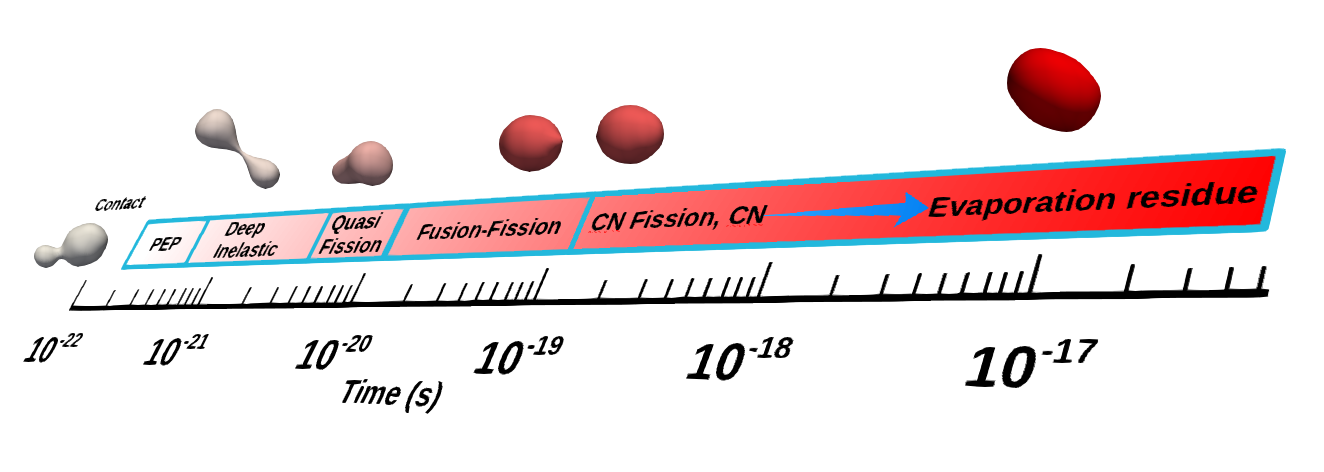
\includegraphics[width=\textwidth]{../Figures/intro_figs/timescale.png}
	\caption{The general timescales of nuclear reactions from quasielastic scattering through fusion and subsequent decay.}
	\label{fig:timescale}
\end{figure}

Our focus is now turned to the dynamics of nuclear physics at low collision energies as predicted by TDHF.
Broadly speaking, for two incoming nuclei with their own distinct numbers of protons and neutrons, one could expect to see a large number of possible outcomes depending on factors such as the orientation of the incoming nuclei, the distance off the collision axis, and the energy between the two fragments.
What is seen experimentally will be some complex combination of initial configurations, however.
The typical technique employed to investigate a given system is then to perform a large number of calculations across the configuration space in an attempt to understand what is happening systematically as you change any initial quantity.
It is for this reason that one must take care to check the full parameter space in order to make authoritative statements on the physics at play in reactions, especially when comparing to experimental data.

The usual method of classifying nuclear reactions is by the length of time that the fragments stay in contact\footnote{The specific definition of contact varies from work to work, though it is typically stated as when the density in the neck region between the nuclei is around half the saturation density, $\rho=0.08$.} before coming apart again.
Of course, if the fragments stay together indefinitely this is interpreted as a fusion event in TDHF.
Though the timescales and definition of reaction channels are fluid, they may be roughly divided into categories as is shown in Fig.~\ref{fig:timescale}.
For reasons mentioned in the previous section TDHF is capable of investigating reaction mechanisms from the far left of the chart up through compound nucleus formation (around $10^{-20}-10^{-19}$s in Fig.~\ref{fig:timescale}).
Any subsequent events after a fused system is formed, like fission or the evaporation of a particle, will not occur in a TDHF calculation and must be dealt with using a separate technique.

\begin{figure}[t]
	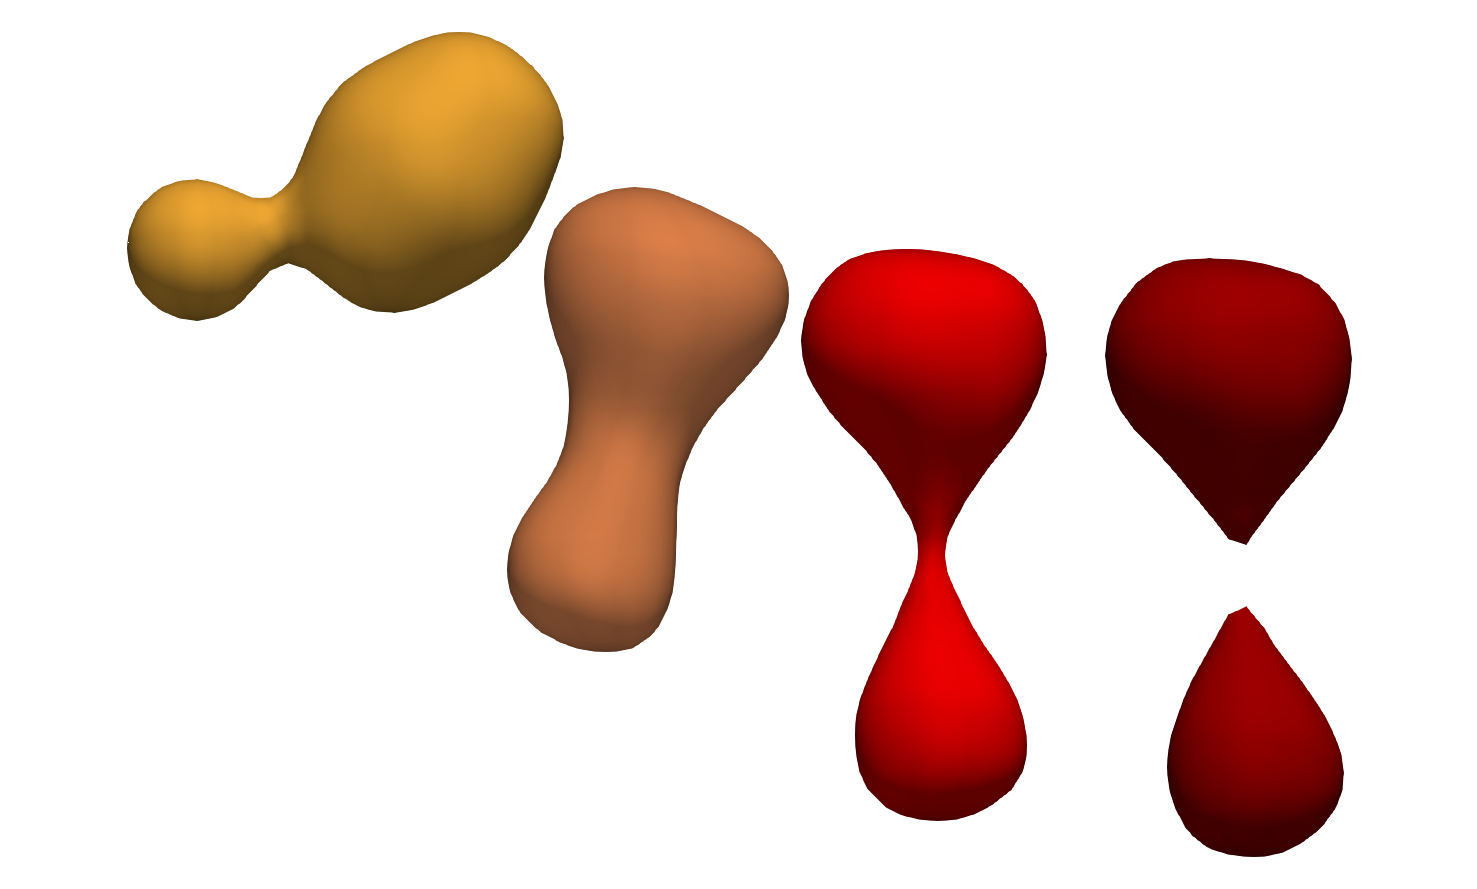
\includegraphics[width=\textwidth]{../Figures/intro_figs/48Ca249BkEvolution_tr.png}
	\caption{A typical density evolution for a quasifission reaction. The system presented is $^{48}$Ca$+^{249}$Bk and the figure is taken from~\citep{godbey2020}.}
	\label{fig:qf}
\end{figure}

As an example case, a typical set of contours from a benchmark quasifission reaction may be seen in Fig.~\ref{fig:qf}.
In this reaction, as is common in quasifission, the initially mass asymmetric system collides and begins to exchange a substantial amount of energy and mass before rotating and forming two new nuclei as they separate.
As mentioned before, the nuclei produced in such a reaction will depend on the initial configuration, and substantial effort has been expended to understand the production rates of nuclei via these sorts of reactions.
From the image it is clear that the dynamics governing the outcome of a nuclear collisions depend on much more than the incoming number of particles, hence the sophisticated tools and techniques used to study these processes.

\section*{Summary}

Through use of state-of-the-art many-body methods this thesis explores nuclear reactions through both theoretical development and extensions of the base theories, as well as through systematic, comprehensive studies of nuclei.
Each chapter either focuses on a specific aspect of nuclear reactions or attempts to exhaustively characterize a given system.
In Chapter~\ref{chapters:chapter_2}, I discuss the development of a new extension to explore the role of transfer in the initial stages of the collision on fusion.
The basis of the technique is described and then select applications are presented to demonstrate the applicability to generic nuclear systems.
Chapter~\ref{chapters:chapter_3} meanwhile continues to focus on fusion, though via a more basic aspect.
Specifically, a method is developed to directly show the impact of the Pauli exclusion principle on heavy ion collisions at low energies.


Chapters~\ref{chapters:chapter_4} and~\ref{chapters:chapter_5} turn away from the development of new extensions to TDHF and instead look into the effect of the Skyrme tensor interaction on fusion for multiple systems.
Similar to this is Chapter~\ref{chapters:chapter_6} which studies fusion cross sections of \textsuperscript{12}C+\textsuperscript{12}C both above and below the fusion barrier.
This study also represents an effort to make extremely precise fusion calculations be checking the effect of numerical changes on the results.

Finally, the last two chapters are largely devoted to transfer studies for two systems of nuclei.
Chapter~\ref{chapters:chapter_7} utilizes direct TDHF collisions to study fragment production in $^{48}$Ca+$^{249}$Bk reactions.
Due to the deformed nature of $^{249}$Bk, a complete sweep of angles was performed to paint the fullest picture yet of quasifission in TDHF.
While also a study of transfer, Chapter~\ref{chapters:chapter_8} goes beyond TDHF to look at fluctuations about the mean field to uncover the correlations that are missing in the base theory.
This system, as did the one before, requires a large amount of computation due to the deformed initial states and the added cost of the beyond TDHF method.




\clearpage
